

%(BEGIN_QUESTION)
% Copyright 2006, Tony R. Kuphaldt, released under the Creative Commons Attribution License (v 1.0)
% This means you may do almost anything with this work of mine, so long as you give me proper credit

Dette reguleringssystemet har problemer med å holde strømningen på et konstant settpunkt. Det reagerer seint på forndringer ved stor strømning og er veldig følsom for forandringer ved lave strømninger. Ut fra P \&ID-en som er vist her, kan du forklare problemet.

$$\includegraphics[width=15.5cm]{mk021x01.eps}$$

\underbar{file mk021.tex}
%\underbar{file i00526.tex}
%(END_QUESTION)





%(BEGIN_ANSWER)

Since the output of a magnetic flowmeter is linear with regard to flow, there is no need for square root extraction, as indicated by the first ``FY'' device in the loop.  Square-rooting the flow signal will only cause problems if there is no need to do so!

%(END_ANSWER)





%(BEGIN_NOTES)

\vskip 20pt \vbox{\hrule \hbox{\strut \vrule{} {\bf Virtual Troubleshooting} \vrule} \hrule}

This question is a good candidate for a ``Virtual Troubleshooting'' exercise.  Presenting the diagram to students, you first imagine in your own mind a particular fault in the system.  Then, you present one or more symptoms of that fault (something noticeable by an operator or other user of the system).  Students then propose various diagnostic tests to perform on this system to identify the nature and location of the fault, as though they were technicians trying to troubleshoot the problem.  Your job is to tell them what the result(s) would be for each of the proposed diagnostic tests, documenting those results where all the students can see.

During and after the exercise, it is good to ask students follow-up questions such as:

\begin{itemize}
\item{} What does the result of the last diagnostic test tell you about the fault?
\item{} Suppose the results of the last diagnostic test were different.  What then would that result tell you about the fault?
\item{} Is the last diagnostic test the best one we could do?
\item{} What would be the ideal order of tests, to diagnose the problem in as few steps as possible?
\end{itemize}


%INDEX% Measurement, flow: magnetic

%(END_NOTES)


